\documentclass{beamer}

\usepackage{epsfig}
\usepackage{multicol}
\usepackage{geometry}
%\usepackage[dvipsnames]{xcolor}
\usepackage{textcomp}
\usepackage{graphicx}
\usepackage{caption}
\usepackage{subcaption}
\usepackage{amsmath}
\usepackage{tcolorbox}
\usetheme{Boadilla}
\usepackage{pict2e}
\usepackage{tikz}
\usepackage{xcolor}


\title[Traitement du signal numérique]{Traitement du signal numérique - HEI4 IMS}
\author[Antony Bazir]{}

\setlength{\unitlength}{1cm}

\begin{document}

\section{Introduction \& Fondamentaux}
\begin{frame}
\centering 
\textbf{Cours : \\ Traitement du signal numérique \\  2024}\\
\vspace{0.5 cm}
Antony BAZIR
\end{frame}

\subsection{Introduction}
\begin{frame}
\frametitle{Traitement du signal}
\textbf{Exemple d'applications ?}
\vspace{0.3cm} 
\begin{columns}[T]

\column{30mm}
\only<2->
{
	\includegraphics[scale=0.2]{micro.png}\\
	\vspace{0.4cm}
	 Signaux analogiques
}
\column{30mm}
\only<3->{
	\includegraphics[scale=0.1]{computers.png}\\
	\vspace{1.2 cm}
	Signaux numériques 
}
\column{30mm}
\only<4->
{
	\includegraphics[scale=0.2]{échographe.png}\\
	\vspace{0.1cm}
	Signaux analogiques et numériques
}
\end{columns}
\end{frame}

\begin{frame}
\frametitle{Notion de filtre}
\textbf{Qu'est ce qu'un filtre ? }\\
\only<2->
{
\vspace{1 cm}
\begin{center}
	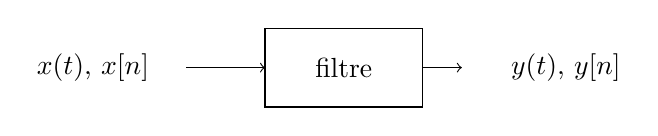
\begin{tikzpicture}

	\draw (2.15,0) node[left] {$x(t)$, $x[n]$};

	
	\draw[->] (2.5,0)-- (3.5,0);
	\draw (3.5,-0.5) rectangle(5.5,0.5) ;
	\draw (4.5,0) node {filtre};

	\draw[->] (5.5,0)-- (6,0);

	\draw (6.5,0) node[right] {$y(t)$, $y[n]$};

	\end{tikzpicture}
\end{center}
}

\only<3->{
\vspace{1 cm}
\begin{block}{}
"En traitement du signal, un filtre est un dispositif ou un processus permettant de retirer des composantes ou des parties indésirables d'un signal." (wikipedia.org)
\end{block}
}
\end{frame}

\subsection{Caractérisation de filtres}
\begin{frame}
\frametitle{Comment caractérise-t-on un filtre ?}
\textbf{Quels termes utiliseriez-vous pour définir un filtre ?}
\vspace{1cm}
\begin{itemize}
\item<2-> Analogique/Numérique
\item<3-> Actifs/Passifs (analogiques)
\item<4-> Causal/Non causal (numériques)
\item<5-> Linéaire/Non linéaire 
\item<6-> Invariant/Non invariant dans le temps
\end{itemize}
\only<7->
{
\begin{block}{}
Objet du cours: Filtres numériques, causaux, linéaires, invariants dans le temps.
\end{block}
}
\end{frame}



\subsection{Linéarité}
\begin{frame}
\frametitle{Notion de linéarité}
\textbf{Question: Que veut dire linéaire en ingénierie des systèmes/automatique/traitement du signal ? \label{linéaire ?} }\\
\vspace{1 cm}
\only<2->
{
Soit $f : x \in \mathbb{R} \rightarrow f(x) \in \mathbb{R} $ et $(x_1,x_2,a,b) \in \mathbb{R}^4$
\\}
\vspace{1 cm}
\only<3->
{
$f$ linéaire si\\
\vspace{0.5 cm}
\begin{block}{}
$f(a x_1 + b x_2) = a f(x_1) + b f(x_2)$ 
\end{block}
}

\end{frame}

\begin{frame}
\frametitle{Notion de linéarité}
 \textbf{Linéarité : application}
\textbf{Soit $x$ une variable réelle, les fonctions suivantes sont-elles linéaires ?}:
 \vspace{0.5cm}
\begin{itemize}
\item<2-> $f(x) = a x^2 + b x + c$ (avec $a$, $b$ et $c$ des constantes réelles positives)
\item<3-> $f(x) = \sqrt{x^2}$
\item<4-> $f(x) = a$ (constante réelle positive)
\item<5-> $f(x) = \ln(x)$
\item<6-> $f(x) = \frac{1}{a x + b}$
\end{itemize}
\vspace{1cm}
\only<8->
{
Aucune de ces fonctions n'est linéaire...
}
\end{frame}

\begin{frame}
\frametitle{Notion de linéarité: capteurs}
\textbf{Que vous évoque la notion de linéarité dans le cadre des capteurs ?}\\
\vspace{1 cm}
\only<2->{
\usetikzlibrary {decorations.pathmorphing} 
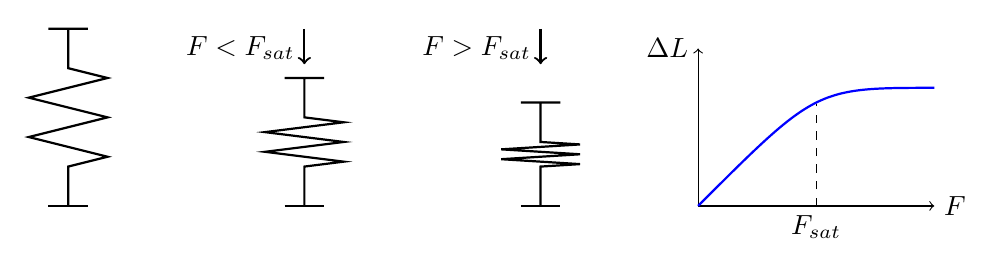
\begin{tikzpicture}

	%spring 
	\draw[thick] (-0.25,0)--(0.25,0);
	\draw[thick] (0,0)--(0,0.5)--++(0.5,0.125) --++(-1,0.25) --++(1,0.25) --++(-1,0.25) --++(1,0.25) --++(-0.5,0.125)--++(0,0.5)--++(-0.25,0)--++(0.5,0); 
		
%			\begin{scope}[xshift = 1.5cm]
%				\draw[thick,<->] (0,2.25)--(0,1.75); 
%				\draw (0,2) node[left] {$\Delta L$};
%			\end{scope}		
		
		
			\begin{scope}[xshift = 3cm]
			\draw[thick] (-0.25,0)--(0.25,0);
			\draw[thick] (0,0)--(0,0.5)--++(0.5,0.125/2) --++(-1,0.25/2) --++(1,0.25/2) --++(-1,0.25/2) --++(1,0.25/2) --++(-0.5,0.125/2)--++(0,0.5)--++(-0.25,0)--++(0.5,0); 
	\end{scope}
	
			\begin{scope}[xshift = 3cm]
				\draw[thick,->] (0,2.25)--(0,1.80); 
				\draw (0,2) node[left] {$F<F_{sat}$};
			\end{scope}	
	
	
	\begin{scope}[xshift = 6cm]
	\draw[thick] (-0.25,0)--(0.25,0);
			\draw[thick] (0,0)--(0,0.5)--++(0.5,0.125/4) --++(-1,0.25/4) --++(1,0.25/4) --++(-1,0.25/4) --++(1,0.25/4) --++(-0.5,0.125/4)--++(0,0.5)--++(-0.25,0)--++(0.5,0); 
	\end{scope}
	
		\begin{scope}[xshift = 6cm]
				\draw[thick,->] (0,2.25)--(0,1.80); 
				\draw (0,2) node[left] {$F>F_{sat}$};
			\end{scope}	
	

	
	\begin{scope}[xshift= 8cm] 
	\draw[->] (0,0)--(3,0) node[right] {$F$};
	\draw[->] (0,0)--(0,2) node[left] {$\Delta L$};	
	\draw[thick,blue] (0,0) .. controls (1.5,1.5) .. (3,1.5);
	\draw[dashed,black] (1.5,0)node[below]{$F_{sat}$} --(1.5,1.3) ;
	\end{scope}
\end{tikzpicture}
}
\only<3->{
\begin{block}{}
Le capteur sort de sa zone de linéarité lorsqu'on perd la relation linéaire/affine entre l'entrée et la sortie
\end{block}
}
\end{frame} 



\subsection{Invariance dans le temps}
\begin{frame}
\frametitle{Notion d'invariance dans le temps}
Prérequis : Notion de retard d'une fonction \\
\only<2->{
\vspace{1 cm} 
Soit $x : t \in \mathbb{R} \rightarrow x(t) \in \mathbb{R} $ \\
\vspace{1 cm} 
La fonction $x(t)$ retardé de $\tau \in \mathbb{R}$ s'écrit $x(t-\tau)$
}

\end{frame}



\begin{frame}
Soit $F$ un filtre de telle sorte que, pour $x(t)$ et $y(t)$ deux fonctions , $ \forall t \in \mathbb{R}, \; y(t) = F(x(t))$ \\

\only<2->
{
\vspace{1cm} 
le filtre $F$  est dit \textbf{invariant dans le temps} si \\
\vspace{1cm}
\begin{center}
$\forall \tau \in \mathbb{R}, \;\; F(x(t-\tau)) = y(t-\tau)$
\end{center}
}

\only<3->
{ 
\begin{block}{}
	En résumé, quelque soit le retard/décalage en entrée, il doit se retrouver en sortie.
\end{block} 
}

\end{frame}

\subsection{Système linéaire et invariant dans le  temps (LIT)}

\begin{frame}
\frametitle{Système linéaire et invariant dans le  temps (LIT) }

Un système F est linéaire invariant dans le temps si :
\begin{itemize}
\item La sortie correspondant à une combinaison linéaire de signaux d'entrée est la combinaison linéaire des signaux de sortie correspondant aux entrées prises séparément\\


\item Quelque soit le retard/décalage, une entrée décalée correspondra à la sortie décalée sans autre différence\\
\end{itemize}

\end{frame} 


\end{document}